\chapter{Implementación}\label{ch:implementacion}

\section{ECJ: Evolutionary Computation for Java}\label{sec:ecj}

Para la implementación del sistema evolutivo se utilizará la plataforma Java ECJ
desarrollada por el Dr. Sean Luke de la universidad de George Mason, diseñada
para la experimentación científica de esta rama \cite{MasonECJ}.

Se caracteriza por ser extremadamente modular y parametrizable. Esta plataforma
consta de diferentes librerías para cubrir casi todos los aspectos de la
computación evolutiva. Nosotros nos centraremos más en las librerías que se
centran en la programación genética.

Se eligió esta plataforma por que una de las normas del concurso es utilizar
Origin, plataforma de desarrollo multiproceso de sistemas evolutivos basada en
ECJ. Al ser una plataforma multiproceso hace que la información que podemos
extraer en las ejecuciones sea mínima. Además, la forma en que se utiliza es
idéntica a Origin con la excepción de unos pocos parámetros de configuración.

La clase principal que tiene ECJ es ec.Evolve. Esta clase se encarga de leer un
fichero de configuración del sistema y empezar la evolución. El fichero de
parámetros sirve para configurar los distintos aspectos de la evolución. Se
encarga tanto de las clases que se utilizarán, como de la estructura de los
árboles del lenguaje de los programas y de muchos otros parámetros de
configuración de las clases que intervienen en el proceso de evolución.

ECJ utiliza una estructura jerárquica de ficheros de configuración, de tal forma
que si queremos utilizar la librería de Koza para la programación genética,
simplemente tendremos que heredar del fichero de configuración de Koza y definir
ciertas propiedades especificas de nuestro problema. Esto se hace mediante la
siguiente línea:

parent.0 = ../../gp/koza/koza.params 

Sin embargo, para tener un control mucho más avanzado y personalizar ciertos
aspectos de nuestro sistema evolutivo necesitamos conocer algunos parámetros que
configuran aspectos cruciales de nuestra aplicación. El resto de parámetros los
encontraremos descritos en el anexo \ref{sec:ecj-params} de este proyecto ya
que es difícil encontrar documentación de estos parámetros.

La jerarquía de ficheros de configuración comienza con el fichero ec.params. Este
fichero configura los parámetros más simples de una ejecución evolutiva como por
ejemplo número de threads del proceso, semillas de números aleatorios, frecuencia
del checkpoint (fotografía de los programas en un punto de la evolución). El
siguiente fichero de la jerarquía es el fichero simple.params. Este fichero
asienta las bases de un proceso evolutivo, concretando las clases que
representarán a nuestros individuos, procesos de evaluación, reproducción,
estadísticas, etc.

El fichero koza.params, es el último fichero antes que el fichero de
configuración concreto de un sistema evolutivo como por ejemplo el nuestro. Este
fichero concreta los aspectos que son necesarios para poder evolucionar
programas. El Dr. Sean se ciñe estrictamente al sistema evolutivo descrito por
Koza \cite{Koza:1992}, no obstante, siempre es posible cambiar el
comportamiento de ciertos módulos para adaptarlos a nuestro sistema.

El sistema de Koza consta de las siguientes características. El fitness será un
número el cual el individuo perfecto adquiere el valor 0 y el peor individuo
tendrá el valor infinito.

Los individuos constarán de un solo árbol de programa. Además este árbol puede
tener restricciones gramaticales.

La forma de reproducción que se va utilizar será una combinación de cruzamiento y
clonación con probabilidades de 0.9 y 0.1 respectivamente. Esto significa que el
operador de reproducción que predominará será el cruzamiento.

Para elegir a los progenitores se utilizará la selección por torneo. Se realizará
un torneo de un número determinado de individuos escogidos aleatoriamente de la
población. El ganador será elegido como padre. La madre será elegida de igual
forma. Para la clonación servirá el mismo método, pero sin cruzamiento.

Para seleccionar el nodo que se intercambiará con el progenitor en el cruzamiento
se limitará la profundidad a un determinado número de nodos, además de elegirse
aleatoriamente dentro del límite establecido. Podremos también condicionar la
búsqueda del nodo eligiendo la probabilidad de seleccionar un nodo terminal, un
nodo no-terminal o incluso la raíz del árbol.

En el proceso de mutación se utilizará “Point Mutation” donde se seleccionará un
nodo aleatorio dentro de una profundidad límite establecida, con un número de
intentos establecido. Una vez que se selecciona el nodo de la misma forma que en
el cruzamiento, se generará un subárbol completamente aleatorio utilizando el
operador grow.

Además en la inicialización de los árboles combinaremos el método grow y el
método full que previamente hemos descrito en el estado del arte.

Una vez descrito el funcionamiento del sistema, explicaremos concretamente los
parámetros principales que utilizaremos a lo largo del proyecto y que nos han
servido para realizar múltiples pruebas:

\begin{itemize}
\item $gp.koza.xover.tries$ : Es el número de intentos que el sistema realiza
para que la operación de cruzamiento se realice con éxito, es decir, sintánticamente correcto. Si no se consigue una combinación adecuada en la operación de cruzamiento se clonarán a los individuos. Por defecto, el número de intentos es 1.
\item $gp.koza.xover.maxdepth$ : Es la profundidad máxima permitida para buscar
subárboles compatibles en ambos individuos para realizar el intercambio en el proceso de cruzamiento. 
\item $select.tournament.size$ : Es el número de individuos que tienen los
torneos del sistema. Cuanto más alto, más probabilidades de escoger al mejor individuo. Sin embargo, cuantas más veces se escoja siempre el mismo individuo, la diversidad empobrecerá.
\item $gp.koza.mutate.tries$ : Número de intentos de mutar a un individuo.
\item $gp.koza.mutate.maxdepth$ : Profundidad máxima para mutar un punto del
árbol de programa. 
\item $gp.koza.grow.min-depth$ y $gp.koza.grow.max-depth$ : La
profundidad máxima que el operador grow utilizará a la hora de generar un árbol estará comprendida entre estos dos valores.
\end{itemize}

\subsection{Origin}\label{subsec:origin}


Origin es el sistema que convierte a ECJ en un sistema multiproceso para ser
utilizado en Frontier. Frontier es un grid de ordenadores alrededor del mundo
desarrollado por Parabon. Para pertenecer a este grid, el único paso a seguir es
instalar la herramienta de Frontier en tu ordenador, y tu ordenador empezará a
formar parte de este grid.

Parabon, la empresa que se encuentra detrás de estas dos tecnologías, combinó la
potencia de investigación de ECJ con la potencia computacional de Frontier, dando
lugar al sistema Origin. Aunque Origin nació de ECJ, actualmente son productos
distintos, mantenidos por empresas diferentes, y cada vez son productos que
divergen más.

Aunque un requerimiento del concurso es utilizar Origin para evolucionar nuestros
programas, tuvimos múltiples problemas desde el inicio: Origin se encuentra en
fases muy tempranas de su desarrollo. Esto hace que ciertos aspectos del sistema
no se encuentran muy desarrollados. Por ejemplo, la ejecución del sistema se
realizaba mediante un script, dificultando utilizar cualquier herramienta de
depuración, al contrario que ECJ, el cual se ejecuta directamente llamando a una
clase Java. Por otro lado, parte del código de Origin esta oculto y no podemos
acceder a él, por lo que es difícil predecir en ciertas ocasiones el resultado de
ciertas acciones. En tercer lugar, en sus últimas versiones dejaron de soportar
el modelo generacional (master-slave), en el cual el ordenador que lanza  la
ejecución se encarga de coordinar el funcionamiento, para soportar exclusivamente
el modelo de estado fijo (oportunistic), donde el comportamiento esta mucho más
distribuido, dificultando enormemente la recogida de estadísticas e información
de funcionamiento del sistema, el cuál es fundamental para el desarrollo de
aplicaciones. Por último, al ser un sistema distribuido, los procesos tienen que
esperar a ser ejecutados según las prioridades de Frontier, por lo que, para
ciertos casos pequeños de prueba el overhead de utilizar un sistema distribuido
es demasiado grande.

Debido a todos estos problemas que presenta Origin decidimos trasladar nuestro
trabajo a ECJ. Gratamente comprobamos que no tuvimos que cambiar prácticamente
nada del código existente. Además ECJ permitía el uso de breakpoints, código
abierto, múltiples hilos de ejecución, ejecución local (podemos inspeccionar
cualquier rincón de nuestro programa) y no dependía de ningún artefacto
prioritario que retrasara la ejecución de nuestros procesos.

Origin es una herramienta orientada a la ejecución: mejora el rendimiento de
nuestra aplicación. No obstante, se encuentra en desarrollo y por lo tanto esta
sujeto a grandes cambios (y fallos), y, por último, resulta muy difícil utilizar
con la herramienta cuando se trata de un trabajo de investigación ya que
necesitamos obtener la máxima información posible de nuestras ejecuciones y
Origin falla en este aspecto.

\subsection{Extensiones a ECJ}\label{subsec:mod-ecj}

Al implementar nuestro sistema tuvimos una serie de problemas que nos obligaron a
realizar ciertas modificaciones a la plataforma ECJ. El problema surgió al
intentar utilizar un lenguaje con fuertes restricciones gramaticales. Estas
restricciones no permiten colocar cualquier nodo como hijo de otro nodo en el
momento de generar árboles. El resultado: desbordando la pila de memoria de la
máquina virtual de Java. Para explicar el motivo del fallo recordemos el método
de generación de árboles full. Este método construía árboles de programa mediante
nodos no-terminales hasta llegar a la profundidad máxima, en donde sólo utilizaba
nodos terminales (vease sección \ref{subsubsec:inittree}). El problema es que en
nuestro lenguaje no siempre es posible colocar un nodo terminal como hijo de otro
nodo. Esto provoca que cuando el método full se encuentra en la fase de colocar
nodos terminales y no encuentra ninguno que pueda utilizar, elige aleatoriamente
entre los nodos no-terminales que gramaticalmente encajan. El desbordamiento de
la pila de memoria se produce al escoger nodos no-terminales que producen que el
árbol se expanda infinitamente. Esto es debido a que el método full desconoce de
antemano qué nodos no-terminales son los que acaban terminando la rama de un
árbol. Es por ello que hay que informar al método full de cuales son los nodos
no-terminales que pueden llevar a terminar la rama de un árbol.

Este es el caso de las funciones de nuestro sistema como move y test. Estas
funciones son símbolos no-terminales que generan sólo un nivel más de profundidad
en la rama del árbol. En este nivel adicional del árbol se encuentran los
argumentos de llamada a la función. Por lo tanto, este tipo de nodos debería
considerarse como un nodo terminal, ya que si se usa este nodo no-terminal, se
producirá la parada de la expansión del árbol.


El sistema no es consciente de estos hechos y por lo tanto no sabe qué nodo
escoger en el caso de que se quiera parar la expansión del árbol solo puede
escoger entre símbolos no-terminales en función de su aridad. En nuestro caso, en
ciertas ocasiones existe el 50\% de posibilidades de que se escoja un símbolo que
puede duplicar el número de nodos o  un símbolo que pare la expansión. Si escoge
el nodo que duplica el número de nodos de la rama, tendrá dos nuevas
oportunidades de volver a escoger el nodo que sigue expandiendo el árbol. Esto
hace muy probable que el sistema cree un árbol infinito, desbordando la memoria
disponible.

La solución consistió en extender la funcionalidad del sistema de tal manera que
desde el fichero de parámetros podamos especificarle qué nodo posee cualidades de
terminal aunque sea no-terminal. Para hacer esto, sobrescribimos la clase GPNode
para leer este flag del fichero de parámetros. Además cambiamos la funcionalidad
de las clases ec.gp.koza.KozaBuilder, ec.gp.koza.HalfBuilder y
ec.gp.koza.GrowBuilder para que tuvieran en cuenta este flag a la hora de
clasificar nodos terminales y no-terminales. De esta forma pudimos generar
árboles sin que se produjera ningún error.

La segunda gran modificación que realizamos en el sistema sirvió para poder
utilizar nuestro propio sistema de fitness. De esta forma, sobrescribiendo la
función que compara dos individuos, podemos decirle al sistema nuestra
preferencia a la hora de elegir.

La ultima modificación es una modificación obligada, es decir, la propia
documentación del framework ECJ recomienda realizar estos cambios. Esta
modificación cambia la manera que tiene el sistema de sacar datos de
funcionamiento e imprimir estadísticas. De esta forma podemos obtener una
información mucho más rica del sistema para poder encontrar la solución a nuestro
problema.

\section{Cubetwister y el cubo de Rubik}\label{sec:cubetwister}


El modelo computacional del cubo de Rubik va a ser el especificado en el concurso. 
Para representar el cubo de Rubik en el ordenador utilizaremos la librería de
Randelshofer (cubetwister.jar) \cite{Randelshofer}, en la versión 1.0.3.2.
Existe una importante diferencia entre la versión 1 y la versión 2, también disponible en la Web,
sobre todo en la nomenclatura de las caras. La numeración de las caras será la
siguiente: la cara frontal será la 0, la derecha, la 1; la inferior, la 2; la
trasera, la 3; la izquierda, la 4; y por último la superior, la 5
(figura \ref{fig:carasrubik}).
 
\begin{figure}[t]
\centering
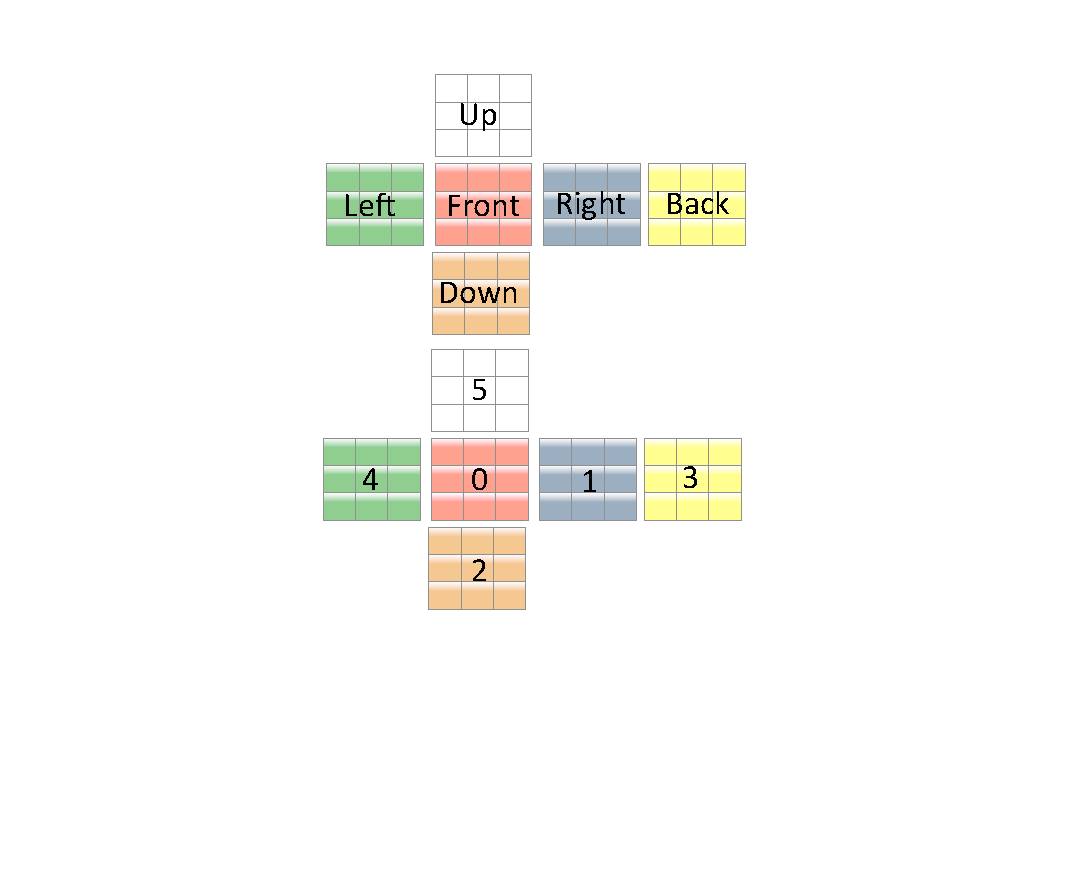
\includegraphics[width=0.55\textwidth]{figs/pdf/carasrubik}
\caption{Asignación numérica de las caras
del cubo de rubik..}
\label{fig:carasrubik}
\end{figure}

Además, internamente, para situarnos dentro de una cara, utilizaremos la
representación gráfica matemática (figura \ref{fig:rubikfaceposition}), donde
X0 e Y0 se situarán en la parte superior izquierda de la cara. No obstante el eje de ordenadas estará invertido, siendo la casilla X0 Y0 la casilla que esta en la esquina superior izquierda y la casilla X2Y2 la casilla de la esquina inferior derecha.

\begin{figure}[t]
\centering
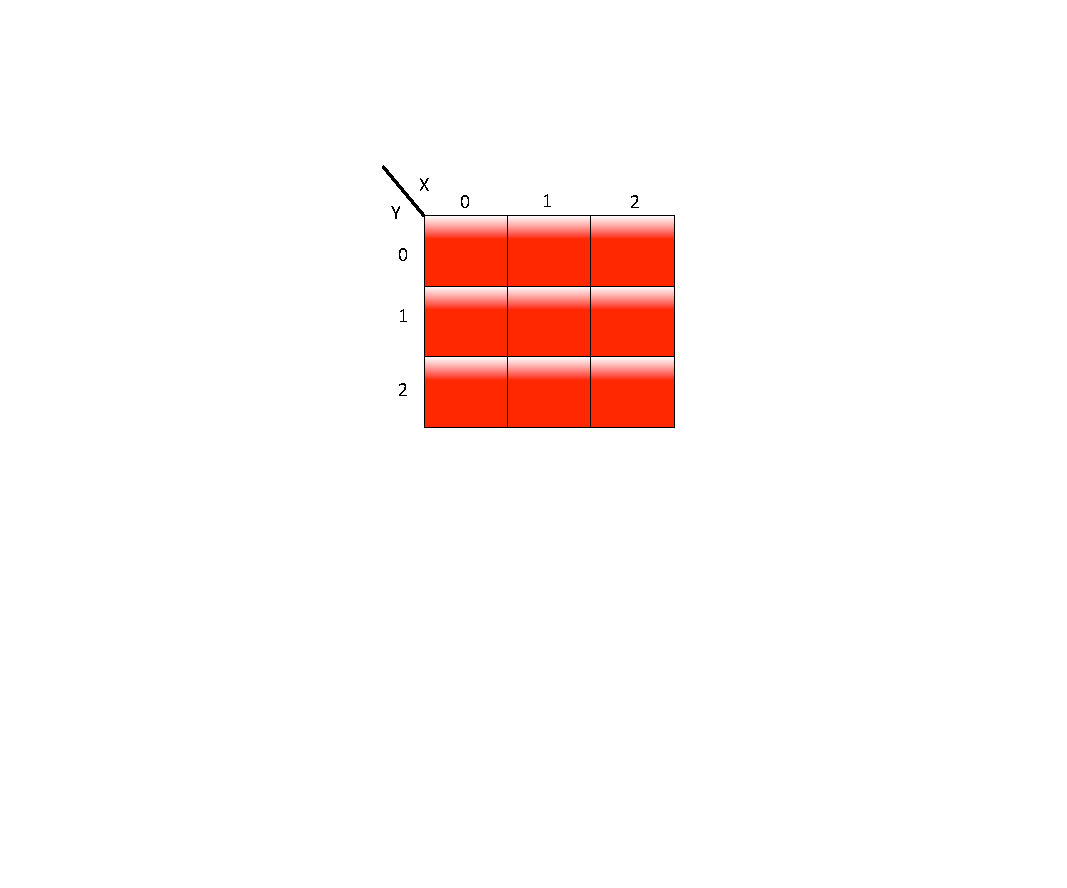
\includegraphics[width=0.45\textwidth]{figs/pdf/rubikfaceposition}
\caption{Asignación numérica de las posiciones de las casillas de una cara
del cubo de rubik.}
\label{fig:rubikfaceposition}
\end{figure}


\clearpage

\section{Diagrama de clases}\label{sec:dia-clases}

Las figuras \ref{fig:package-rubik}, \ref{fig:package-direction},
\ref{fig:package-color} y \ref{fig:package-func} representan los diagramas de
clase de la aplicación.

\begin{figure}[bct]
\centering
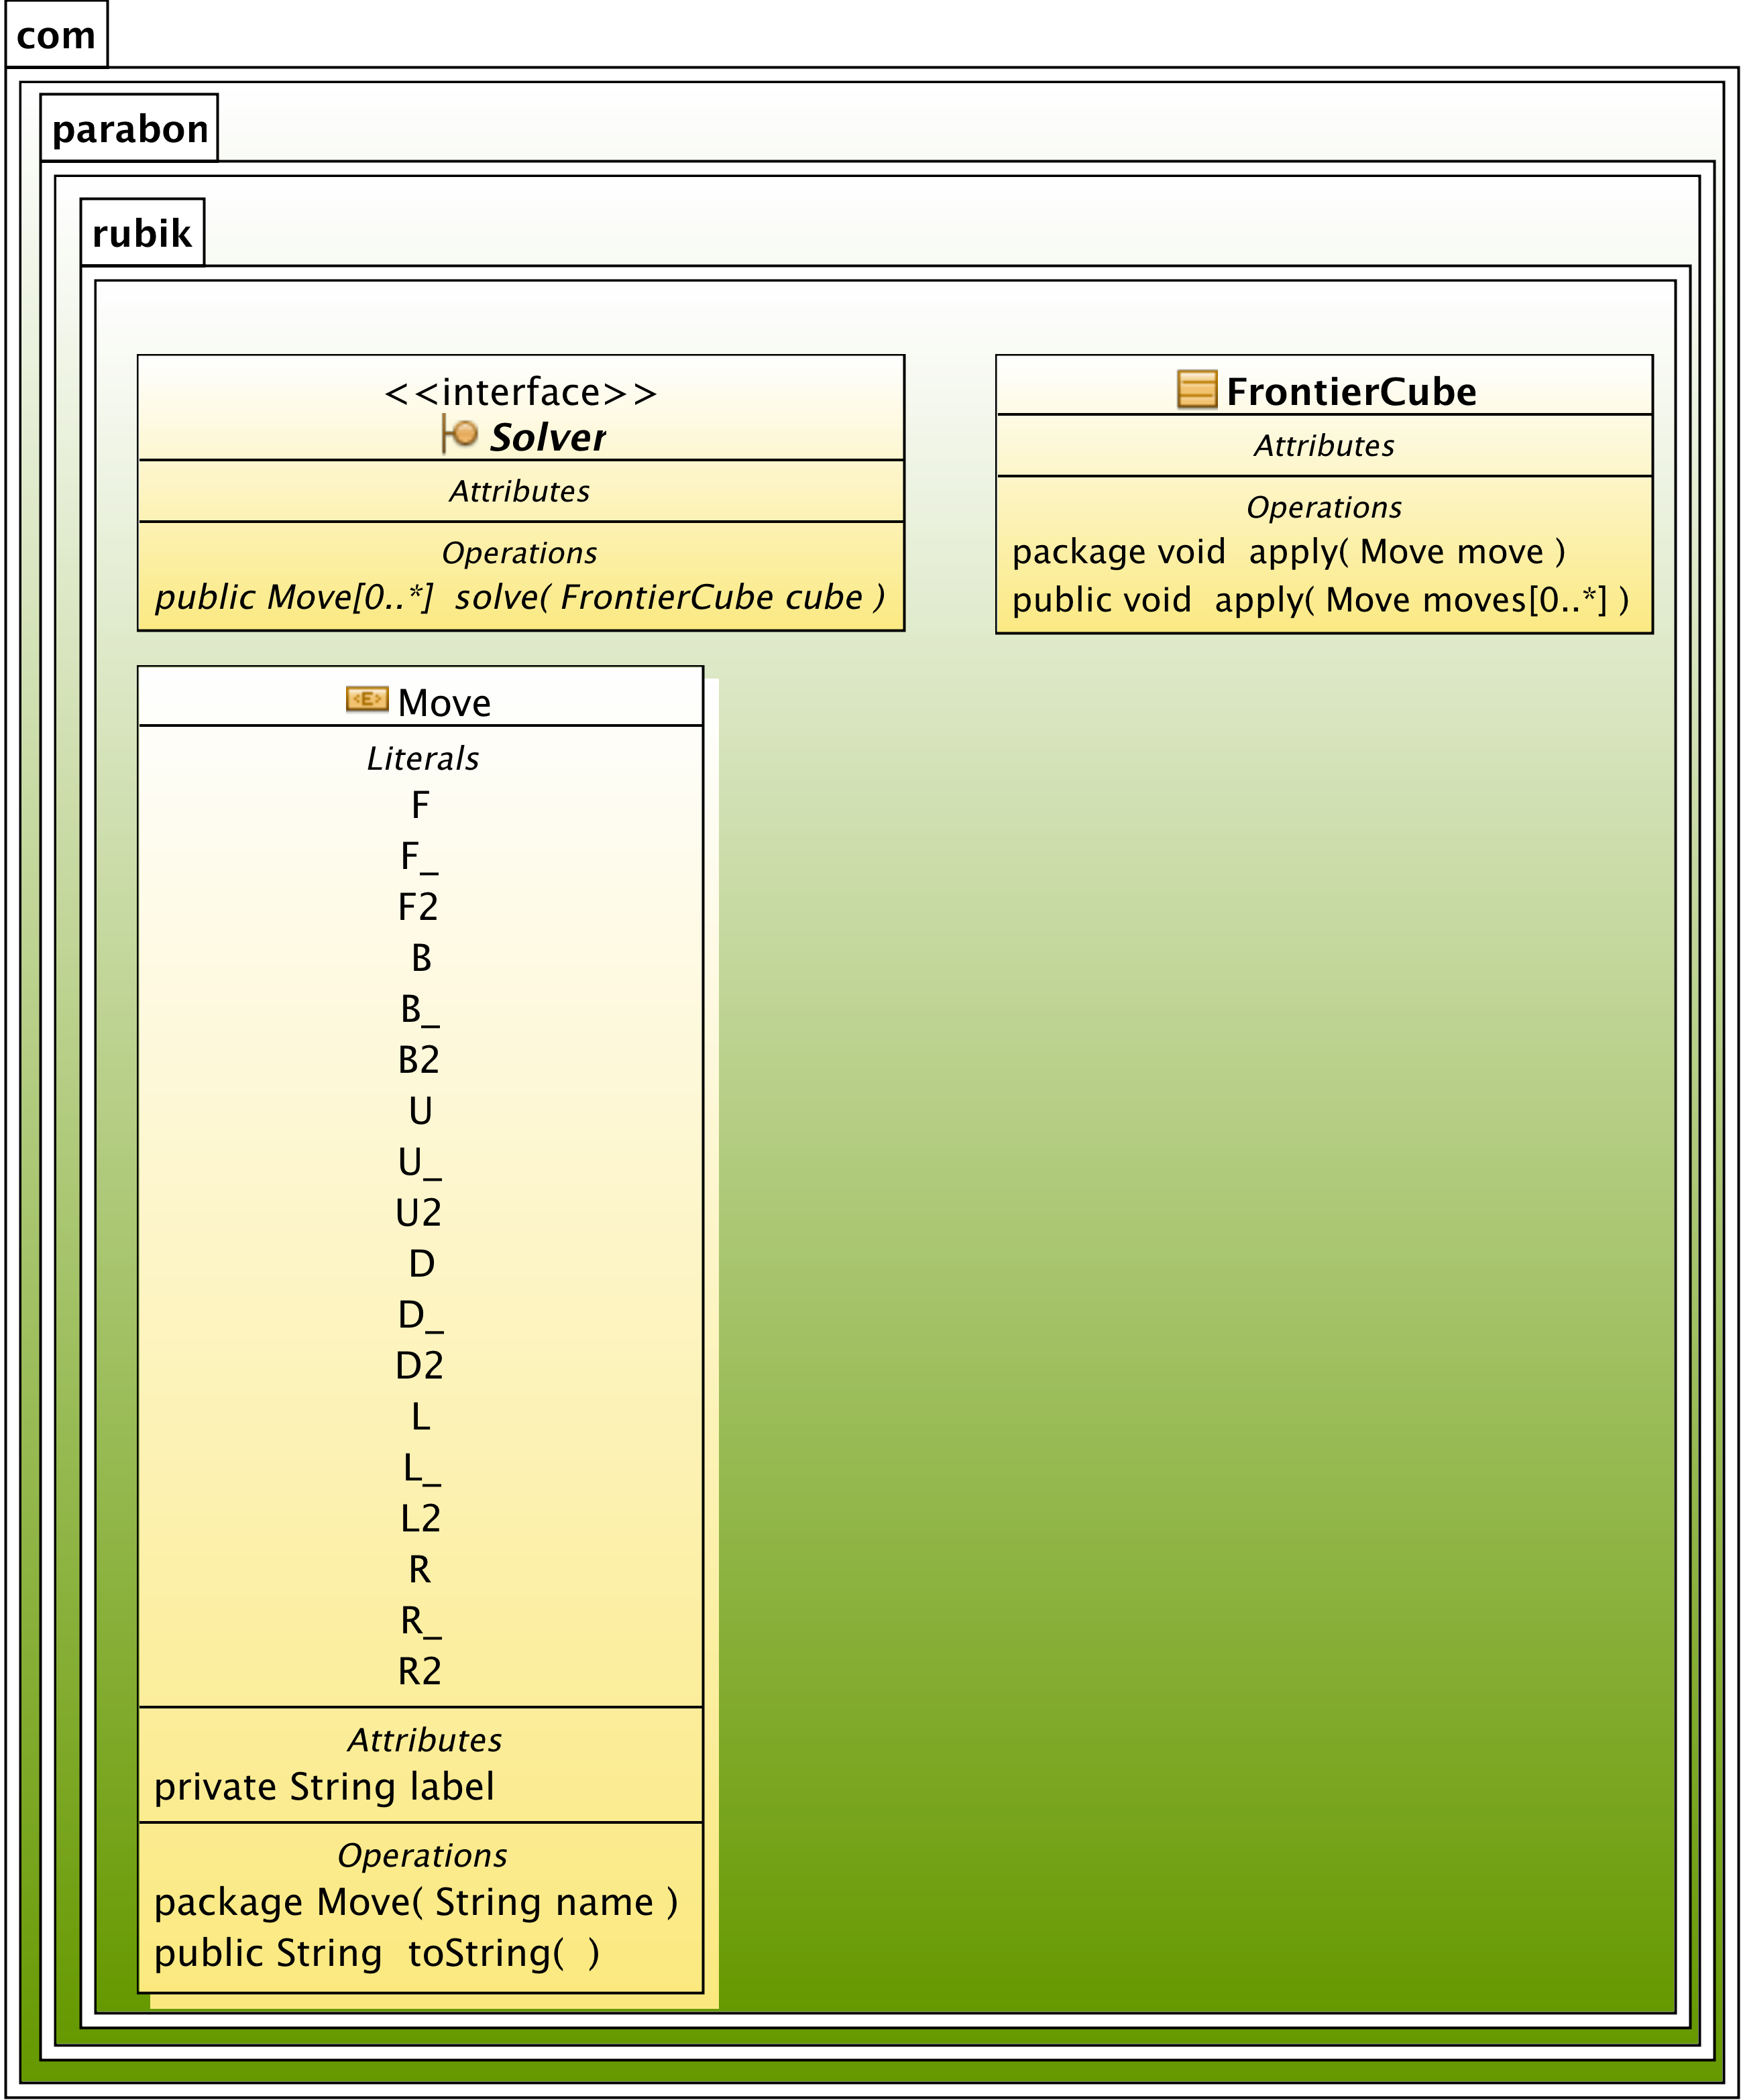
\includegraphics[scale=0.10]{figs/classes/rubik}
\caption{Paquete com.parabon.rubik}
\label{fig:package-rubik}
\end{figure}

\begin{figure}[cbt]
\centering
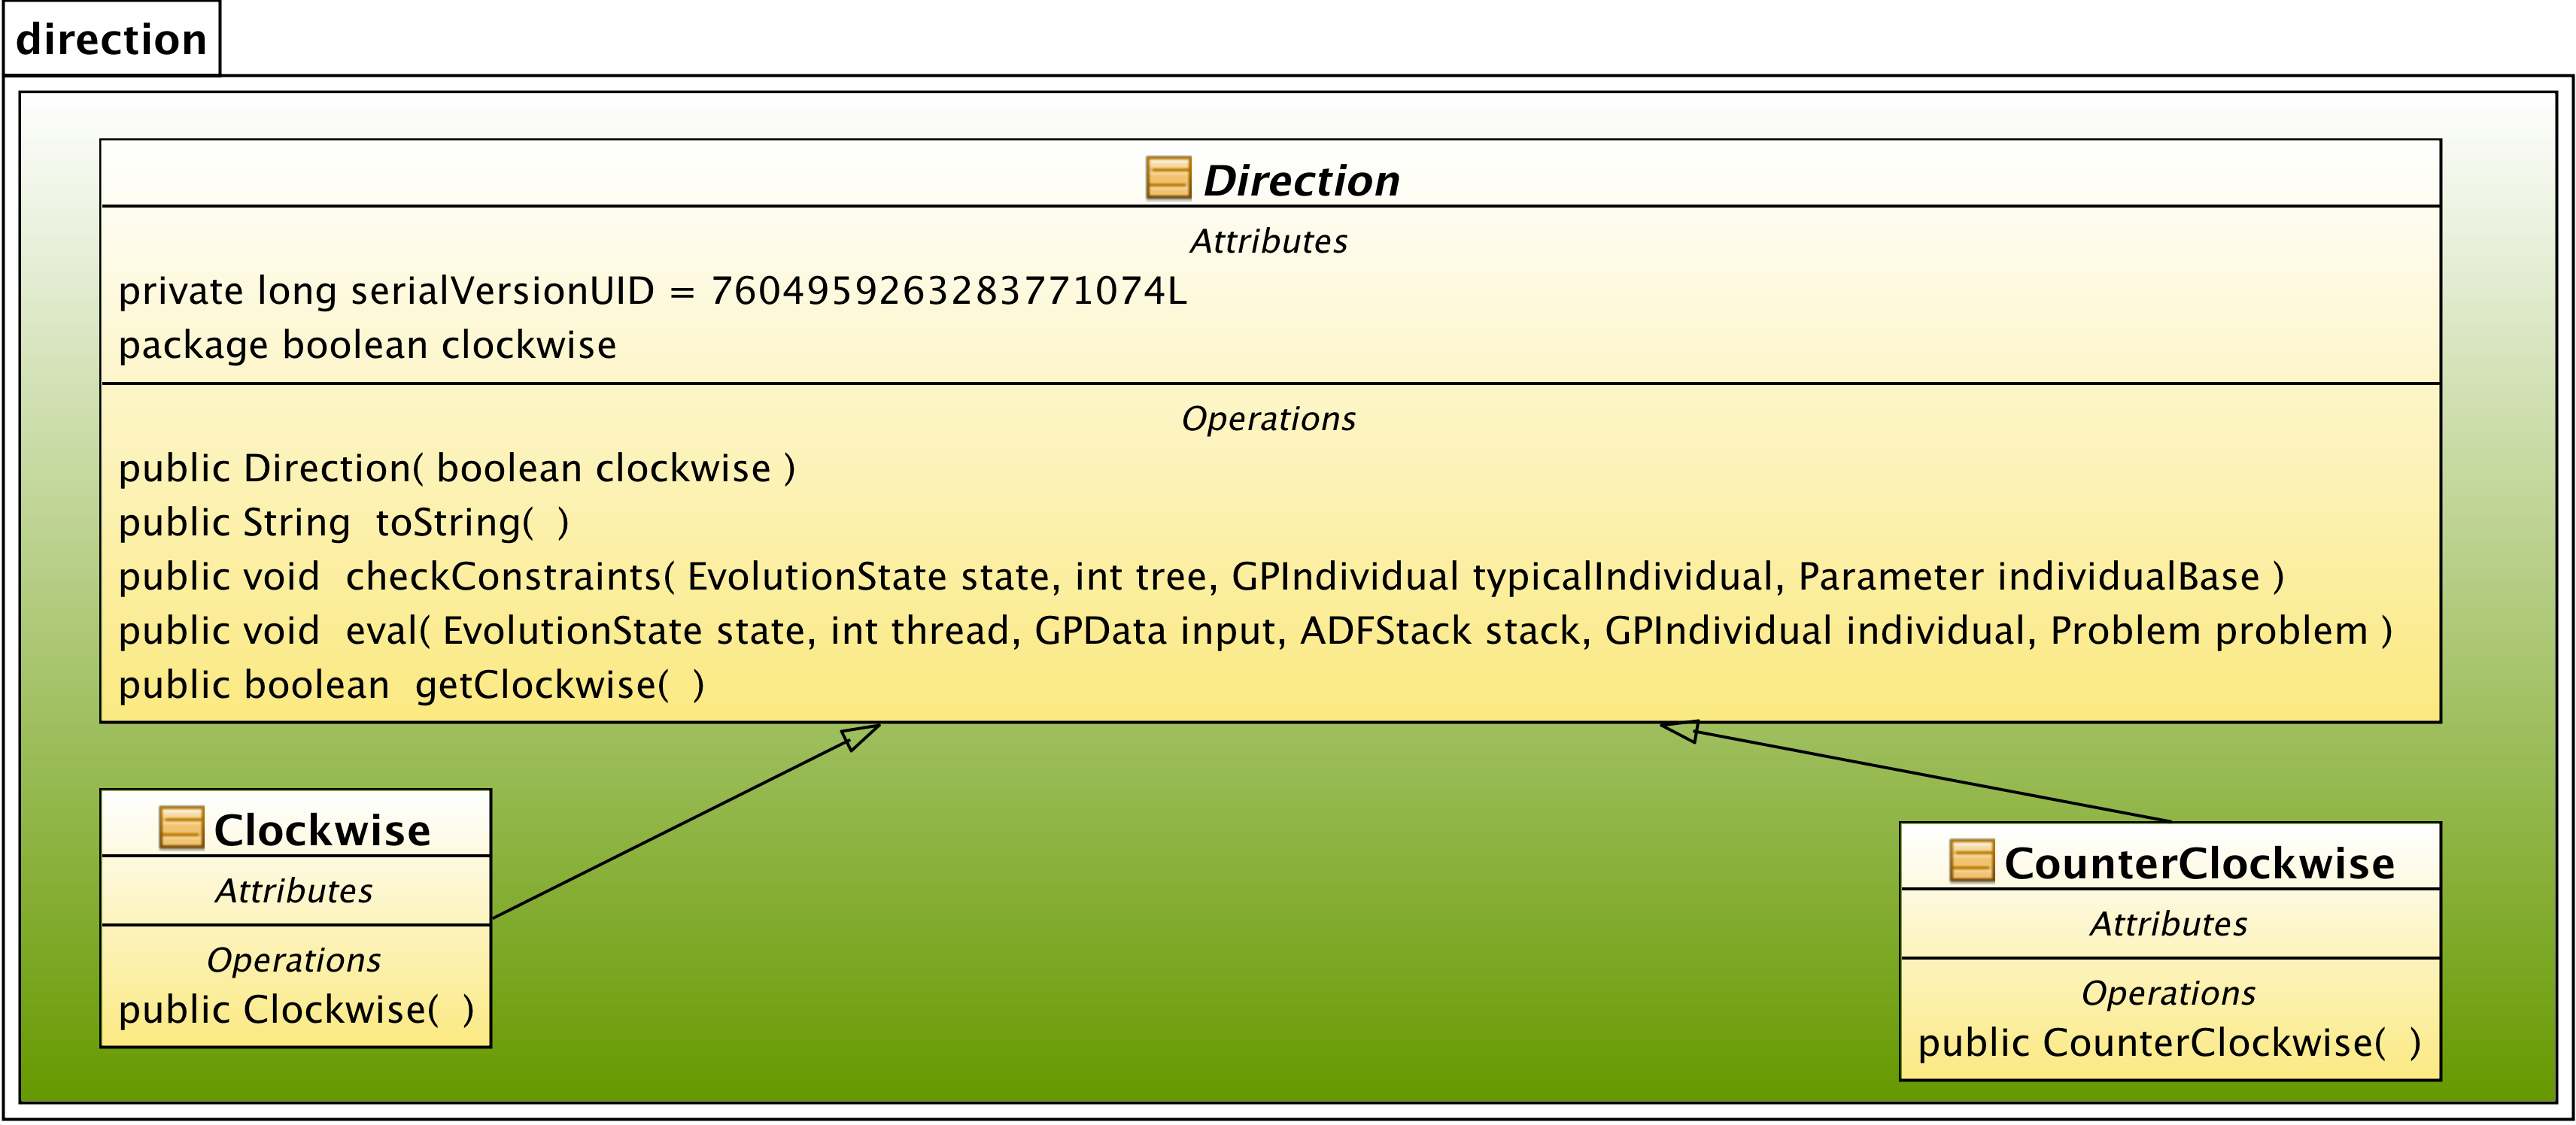
\includegraphics[scale=0.12]{figs/classes/direction}
\caption{Paquete direction.}
\label{fig:package-direction}
\end{figure}

\begin{figure}[ctb]
\centering
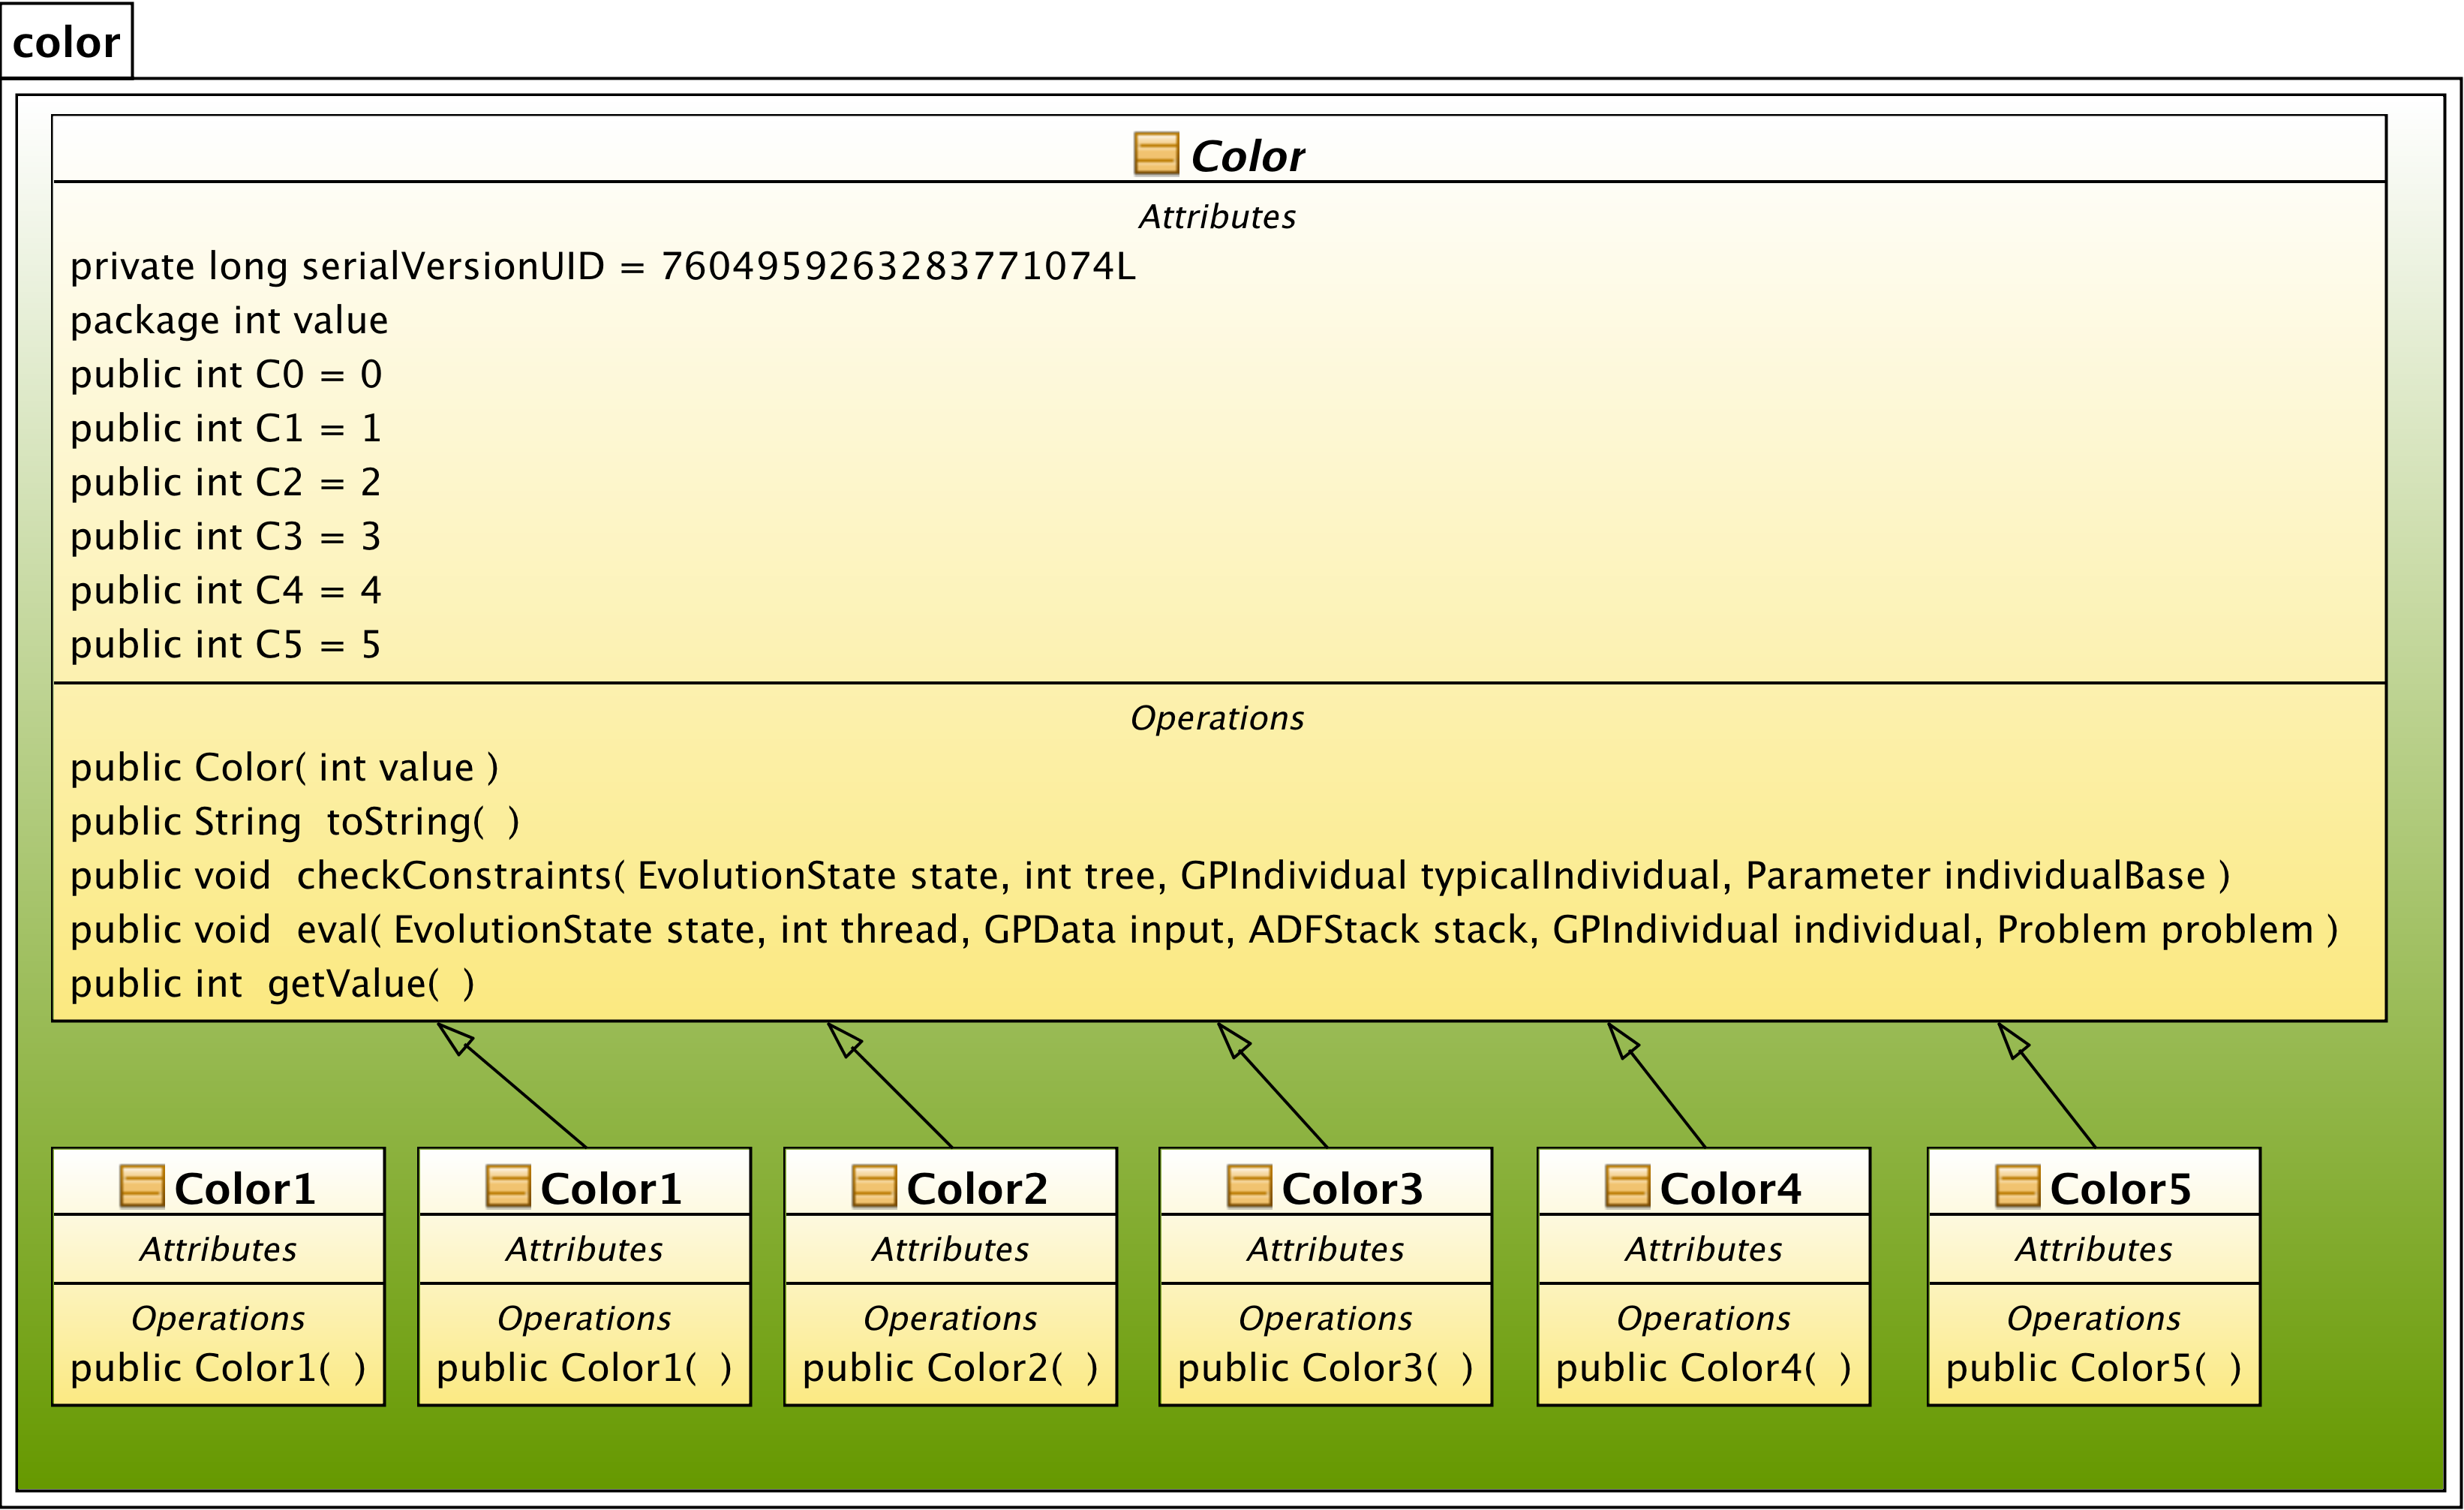
\includegraphics[scale=0.12]{figs/classes/color}
\caption{Paquete color.}
\label{fig:package-color}
\end{figure}

\begin{figure}[cbt]
\centering
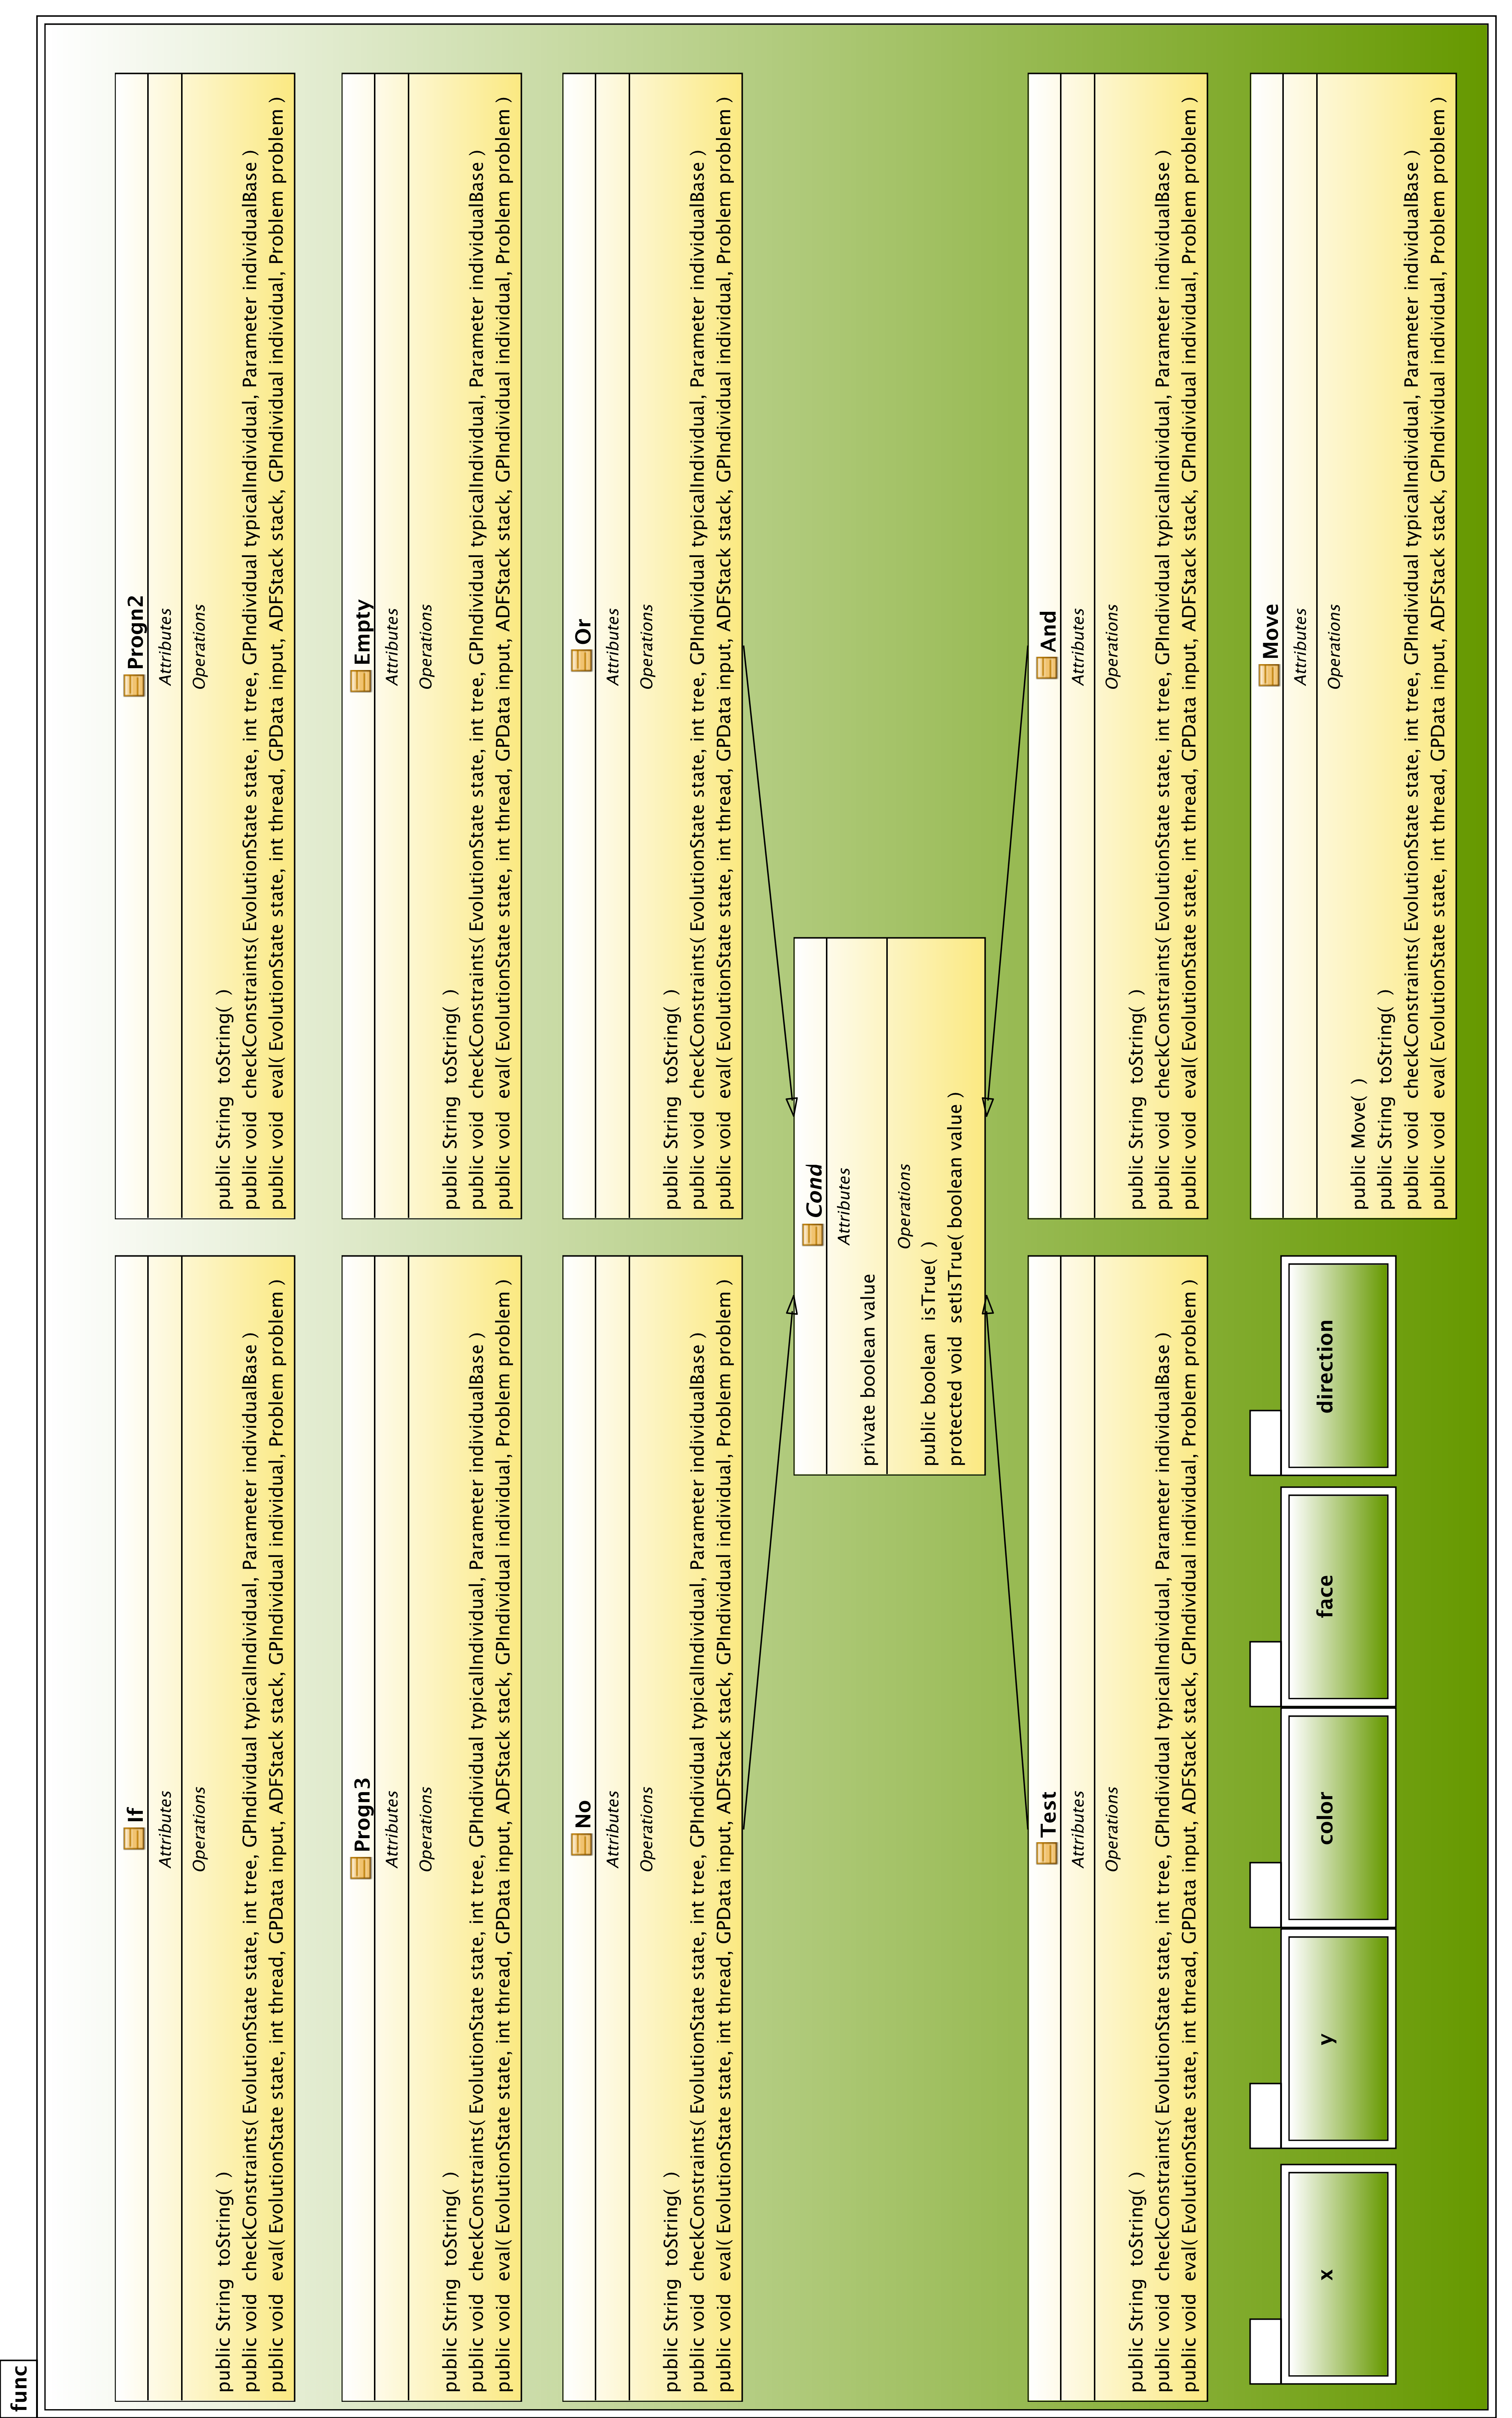
\includegraphics[scale=0.09]{figs/classes/func}
\caption{Paquete func.}
\label{fig:package-func}
\end{figure}

